\documentclass[12pt, a4paper]{article}
\usepackage{amsmath, amssymb, amsfonts} 
\usepackage{inputenc}
\usepackage{float}
\usepackage{graphics}                 
\usepackage{color}                    
\usepackage{hyperref}
\usepackage{ptext}
\usepackage{graphicx}                         
%\settextfont[Scale=.9]{Calibri}

%\graphicspath{ {images/} }

\hypersetup{
	colorlinks=true,
	linkcolor=blue,
	filecolor=magenta,      
	urlcolor=cyan
}


\title{
	{\Huge \textbf{In the name of God}}
	\\[20pt]
	
\includegraphics[width=0.5\linewidth]{../assets/IUST_logo_color_eng.jpg} \\
	{\normalsize Department of Computer Engineering}
}

\author{
	\\[10pt]
	\textbf{{\LARGE Natural Language Processing}}
	\\[10pt]
	\LARGE Final Phase Report
	\thanks{\url{https://github.com/yegmor/NLPProject}}
	
	\\[30pt]
	\textbf{Yeganeh Morshedzadeh}
	\\[5pt]
	Student Number: 96521488
}

\date{Spring 2021} 

\begin{document}
	
\maketitle
%\graphicspath{{../reports/images}}‎
	
\clearpage
%\addtocontents{toc}{\textbf{Content}~\hfill\textbf{Page}\par}
\tableofcontents
\newpage

\listoffigures
\newpage

\listoftables
\newpage

\begin{abstract}
	In this project, we tried to use Natural Language Processing to better understand Depression and Anxiety posts. The dataset is gathered from Reddit communities \href{https://www.reddit.com/r/depression}{r/depression} and \href{https://www.reddit.com/r/Anxiety}{r/Anxiety}.
	\\[10pt]
	
	For this project, at first, we wrote a project proposal (\href{https://docs.google.com/document/d/1tHGEmEgn8-sp8MD72d8NjnZsq-GpVupzsMWgnqaGi-Y/edit?usp=sharing}{Google Docs}), and afterwards, in the first phase (\href{https://docs.google.com/document/d/1Jc2ELhweU01Tbf0WalU7wVQABdAV4w50mhQnmMpU2mM/edit?usp=sharing}{Google Docs}), we gathered data and made some exploratory data analysis. 
	\\[10pt]
	
	In the final phase, we went deeper, and tried various NLP tasks, such as, computing Word2Vec, Tokenization, Parsing, and creating a language model based on our the dataset.
\end{abstract}

\newpage
\part{Word2Vec}
\large{\textbf{Filename:} 3\_word2vec.ipynb}

\section*{Code}
We use Gensim implementation of word2vec: https://radimrehurek.com/gensim/models/word2vec.html

For this part we have three Word2Vec models, named as dep\_w2v\_model, anx\_w2v\_model, and all\_w2v\_model. Moreover, with boolean parameters, load and save, the model will be saved and/or loaded in the my\_word2vec function.


\begin{table}[ht]
	\caption{Word2Vec vocabulary size} 
	\centering 
	\vspace{5mm} 
	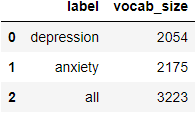
\includegraphics[width=0.5\linewidth]{../reports/images/w2v_vocab-size.png}
	\label{table:nonlin} 
\end{table}



\section*{Results and Examples}
In this part, we used t-SNE visualization. t-SNE is a non-linear dimensionality reduction algorithm that attempts to represent high-dimensional data and the underlying relationships between vectors in a lower-dimensional space.

To make the visualizations more relevant, we will look at the relationships between a query word (in \textcolor{red}{**red**}), its most similar words in the model (in \textcolor{blue}{**blue**}), and other words from the vocabulary (in \textcolor{green}{**green**})

\begin{figure}[H]
	\centering{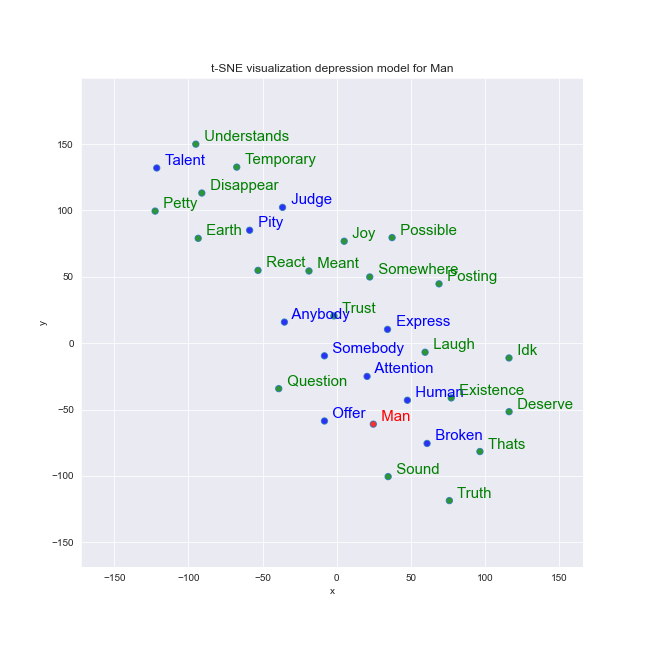
\includegraphics[width=\linewidth, height=\textheight, keepaspectratio]{../reports/images/word2vec_depression_man.png}}
	\caption{t-SNE visualization for man}
	\label{word2vec_depression_man}
\end{figure}

\newpage
\part{Tokenization}
\large{\textbf{Filename:} 4\_tokenization.ipynb}

\section*{Code}
In this part, we have used KFold to split our data into train and test. Afterwards, we train SentencePiece model based on the data. Lastly, we compute <UNK> on our test dataset. 

\section*{Results and Examples}


\newpage
\part{Parsing}
In this part, we used Stanza, which is a a Python NLP Package, and a collection of accurate and efficient tools for the linguistic analysis of many human languages. Starting from raw text to syntactic analysis and entity recognition, Stanza brings state-of-the-art NLP models to languages of your choosing.

More specifically, we used their \href{http://stanza.run/}{Online Demo} to create a manual .CoNLL file based on our dataset. Later, we can use \href{https://universaldependencies.org/conllu_viewer.html}{Universal Dependencies CoNLL viewer} to automatically generate parse tree from .CoNLL file.

\section*{Results and Examples}

The reported Unlabeled Attachment Score (UAS) on our test file was 86.05.

\begin{figure}[H]
	\centering{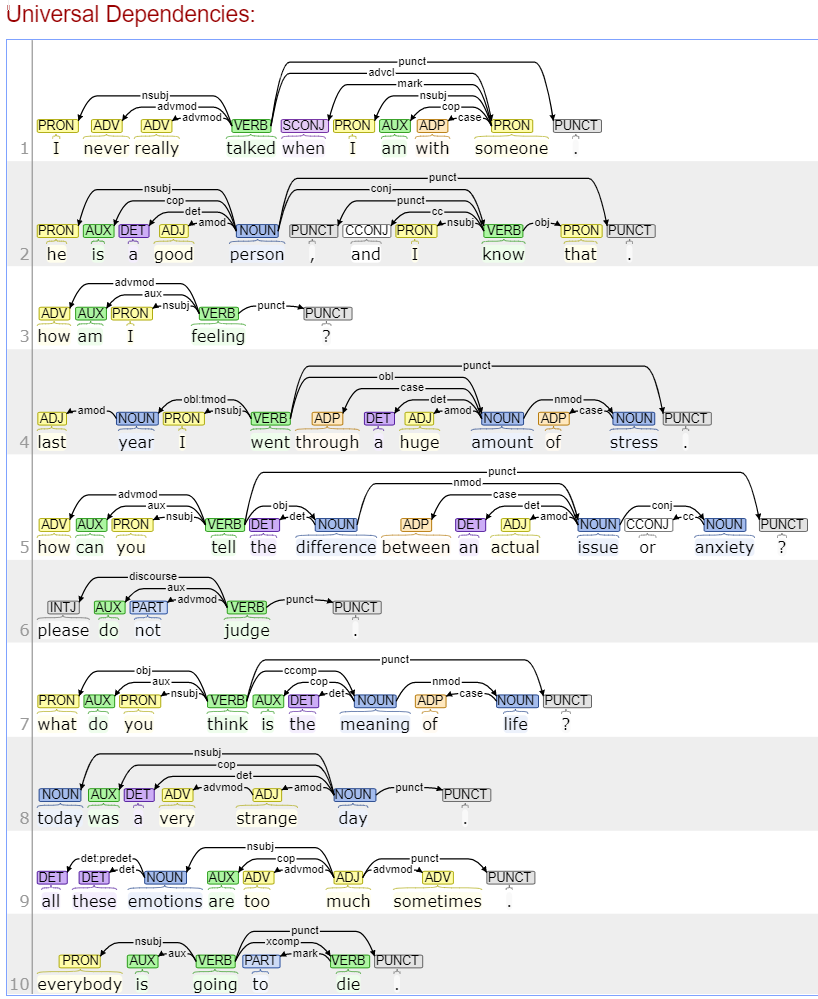
\includegraphics[width=\linewidth, height=\textheight, keepaspectratio]{../reports/images/parsing_examples_UDtree.png}}
	\caption{Universal Dependencies for 10 sentences}
	\label{parsing_examples}
\end{figure}

\begin{enumerate}
	\item I never really showed any sadness when I am with someone.
	\item he is a good person, and I know that.
	\item how am I feeling?
	\item last year I went through a huge amount of stress.
	\item how can you tell the difference between an actual issue or anxiety?
	\item please do not judge.
	\item what do you think is the meaning of life?
	\item today was a very strange day.
	\item all these emotions are too much sometimes. 
	\item everybody is going to die.
\end{enumerate}

\newpage
\part{Language Model}
\large{\textbf{Filename:} 5\_language-model.ipynb}

In this part, we have develop a model of the text that we can then use to generate new sequences of text.

\section*{Code}
We will start by preparing the data for modeling. 
We have picked a length of 50 words for the length of the input sequences, and we have attached 1 output word at the end of the sequences. Afterwards, we save the long list of sequences.


For our language model, after loading our dataset, we used an Embedding Layer to learn the representation of words, and a Long Short-Term Memory (LSTM) recurrent neural network to learn to predict words based on their context. More precisely, we have used a two LSTM hidden layers with 100 memory cells each. Following, we have a dense fully connected layer with 100 neurons connects to the LSTM hidden layers to interpret the features extracted from the sequence.

After the model is trained, we use generate\_seq function that takes as input the model, the tokenizer, input sequence length, the seed text, and the number of words to generate. 

\section*{Results and Examples}
\begin{figure}[H]
	\centering{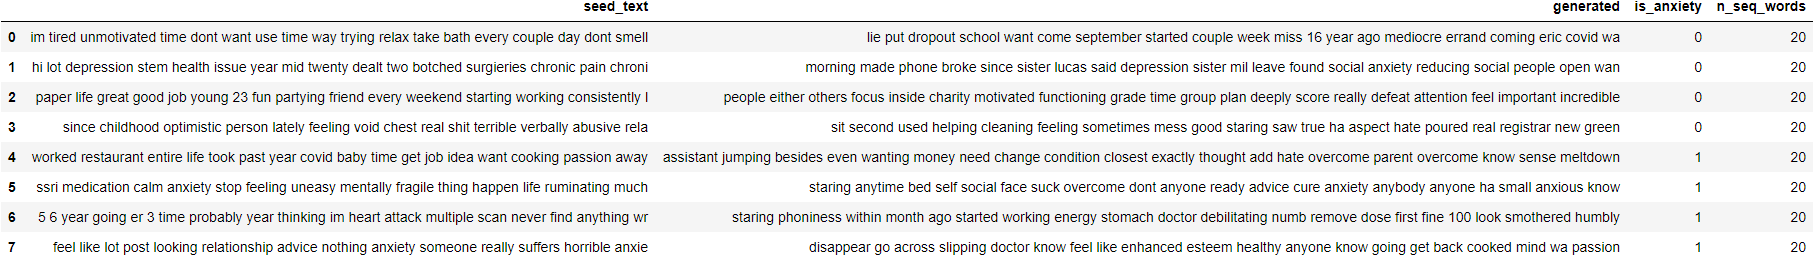
\includegraphics[width=\linewidth, height=\textheight, keepaspectratio]{../reports/images/normal-lm_examples.png}}
	\caption{Examples for simple language model}
	\label{normal-lm_examples}
\end{figure}


\newpage
\part{Fine-tuning}

\section*{Classification}
\large{\textbf{Filename:} 6\_finetune\_classification.ipynb}

\subsection*{Code}

\begin{figure}[H]
	\centering{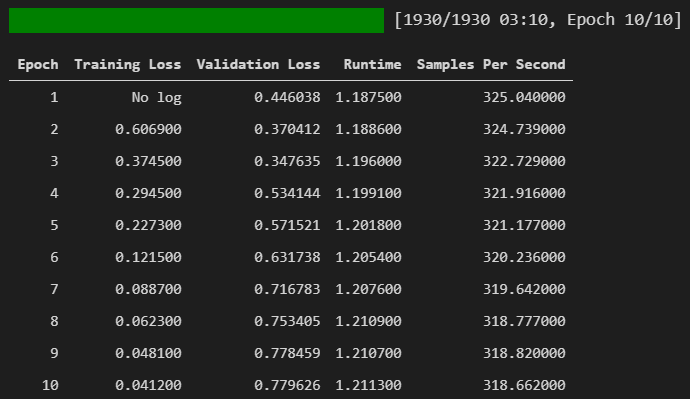
\includegraphics[width=\linewidth, height=\textheight, keepaspectratio]{../reports/images/classification-lm_train.png}}
	\caption{Training bert classification language model}
	\label{classification-lm_train}
\end{figure}

\begin{figure}[H]
	\centering{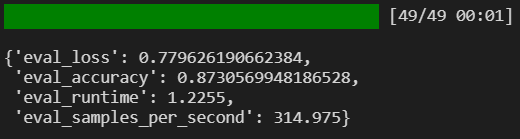
\includegraphics[width=\linewidth, height=\textheight, keepaspectratio]{../reports/images/classification-lm_eval.png}}
	\caption{Evaluating bert classification language model}
	\label{classification-lm_eval}
\end{figure}

\subsection*{Results and Examples}
\begin{figure}[H]
	\centering{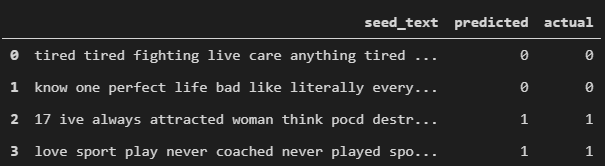
\includegraphics[width=\linewidth, height=\textheight, keepaspectratio]{../reports/images/classification-lm_examples.png}}
	\caption{Examples for bert classification model}
	\label{classification-lm_examples}
\end{figure}


\section*{Language Model}
\large{\textbf{Filename:} 7\_finetune\_language-model.ipynb}

In this part, we have used our Reddit dataset to fine-tune our distilgpt-2.

For this purpose, we first prepare the dataset and build a TextDataset, load the pre-trained GPT-2 model and tokenizer, initialize Trainer with TrainingArguments, and finally, train and save the model. 

\subsection*{Code}
The TextDataset is a custom implementation of the Pytroch Dataset class implemented by the transformers(4.2.2) library.
\\Also, we have used the tokenzier from the distilgpt-2 model on huggingface.
\\Afterwards, we initialize Trainer class that provides an API for feature-complete training, and we set the Hyperparameters we are going to use in the TrainingArguments.

\subsection*{Results and Examples}
\begin{figure}[H]
	\centering{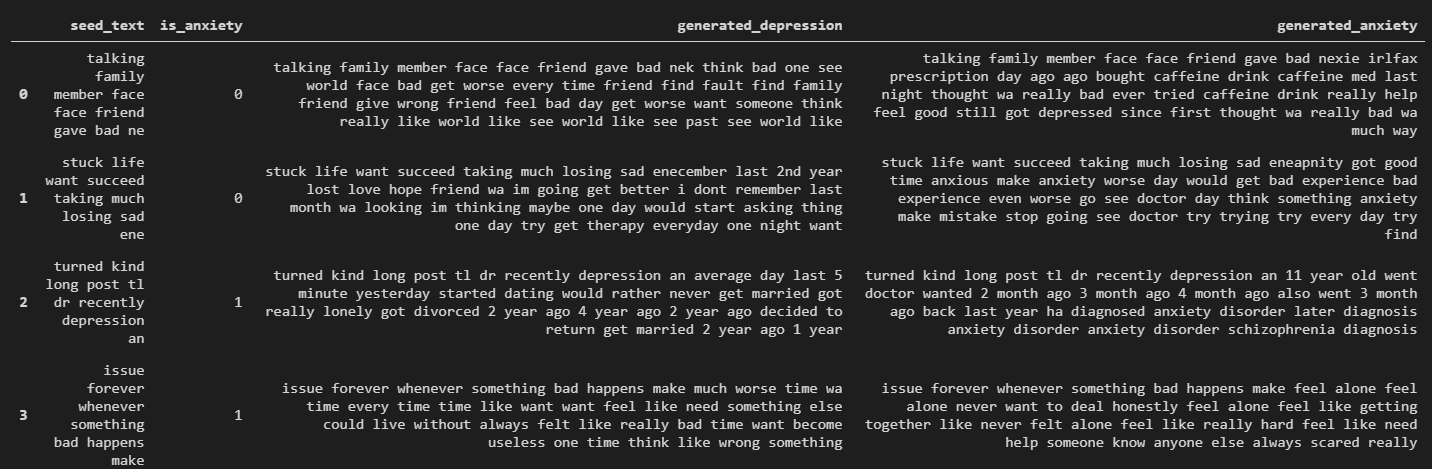
\includegraphics[width=\linewidth, height=\textheight, keepaspectratio]{../reports/images/finetune-lm_examples.png.png}}
	\caption{Examples for distilgpt2 language model}
	\label{finetune-lm_examples.png}
\end{figure}
%
%\begin{figure}[H]
%	\centering{\includegraphics[width=\linewidth, height=\textheight, keepaspectratio]{images/table.png}}
%	\caption{جدول به ازای مقادیر مختلف n}
%	\label{table}
%\end{figure}


\newpage



\begin{thebibliography}{9}
	\bibitem{bib0}
	\url{https://towardsdatascience.com/goodbye-world-4cc844197d51}
	
	\bibitem{bib1}
	\url{https://colab.research.google.com/github/google/sentencepiece/blob/master/python/sentencepiece_python_module_example.ipynb#scrollTo=ee9W6wGnVteW}
	
	\bibitem{bib2}
	\url{https://gmihaila.github.io/tutorial_notebooks/gpt2_finetune_classification/}
	
	\bibitem{bib3}
	\url{https://colab.research.google.com/github/philschmid/fine-tune-GPT-2/blob/master/Fine_tune_a_non_English_GPT_2_Model_with_Huggingface.ipynb}
	
	\bibitem{bib4}
	\url{https://github.com/huggingface/notebooks/blob/master/examples/language_modeling.ipynb}
	
	\bibitem{bib5}
	\url{https://www.kaggle.com/pierremegret/gensim-word2vec-tutorial}
	
	\bibitem{bib6}
	\url{https://machinelearningmastery.com/how-to-develop-a-word-level-neural-language-model-in-keras/}
	
	\bibitem{bib7}
	\url{https://huggingface.co/transformers/training.html}
	
	\bibitem{bib8}
	\url{https://www.kaggle.com/achintyatripathi/gensim-word2vec-usage-with-t-sne-plot}
	
	\bibitem{bib9}
	\url{https://colab.research.google.com/github/borisdayma/huggingtweets/blob/master/huggingtweets-demo.ipynb}
	
	\bibitem{bib10}
	\url{https://huggingface.co/transformers/custom_datasets.html}
	
	\bibitem{bib11}
	\url{https://colab.research.google.com/github/google/sentencepiece/blob/master/python/sentencepiece_python_module_example.ipynb#scrollTo=-k5KbVgiYae-}
	
\end{thebibliography}

\end{document}          
